\documentclass[12pt,a4paper]{article}

\usepackage[utf8]{inputenc}
\usepackage[english]{babel}

\usepackage[pdftex]{graphicx}
\usepackage[top=1in, bottom=1in, left=1in, right=1in]{geometry}
\usepackage{amsmath}
\usepackage{booktabs}
\usepackage{xcolor}

\linespread{1.06}
\setlength{\parskip}{8pt plus2pt minus2pt}

\widowpenalty 10000
\clubpenalty 10000

\newcommand{\HRule}{\rule{\linewidth}{0.5mm}}

% Marks a value that only exists once the bench data is captured. Anything still
% red on the day of submission is not finished.
\newcommand{\gap}[1]{\textcolor{red}{[\textnormal{#1}]}}

\usepackage[hidelinks]{hyperref}

\begin{document}

\begin{titlepage}
\begin{center}


\includegraphics[width=0.3\textwidth]{UCTLOGO.png}~\\[2cm]

\HRule \\[0.4cm]
{ \LARGE
  \textbf{Lab 1 Report}\\[0.4cm]
  \emph{System Identification}\\[0.4cm]
}
\HRule \\[1.5cm]

{ \large
  Tri Tac Le\\[0.2cm]
  EEE3094S Control Systems Engineering\\[0.2cm]
  LXXTRI004
}

\vfill

\textsc{\large Mechatronics: Department of Electrical Engineering}\\[0.4cm]
{\large \today}

\end{center}
\end{titlepage}

\tableofcontents
\newpage
\setcounter{page}{1}

\section{Introduction}\label{sec:intro}

The suspension of the simulated F-34B is a spring, mass and damper system whose spring
constant and damping constant are generated from my student number, so the plant is
unknown before the experiment and cannot be looked up. The aim of this lab is to recover a
transfer function for that plant from measurements alone, which is what system
identification means in practice: choose inputs that make the unknown parameters visible in
the output, then read those parameters off the response.

Two experiments are used because each one exposes a different part of the model. A step
input shows the transient directly, so the steady state gain, the presence or absence of
oscillation, and the damped period can be read from a single log. A set of sinusoidal
inputs samples the frequency response, which fixes the corner frequency and the phase
behaviour, and gives an independent check on the values taken from the step. Where the two
disagree, that disagreement is itself a result and is reported as such.

Section~\ref{sec:modelling} derives the model structure from the equation of motion given
in the brief, and states which measurable feature of a response determines which parameter.
Section~\ref{sec:system_id} applies that to the measurements. Section~\ref{sec:validation}
simulates the identified model and compares it against the same data it was built from.

\section{System Modelling}\label{sec:modelling}

\subsection{System Model}

\subsubsection{Differential equation describing the motion of the mass}

The brief describes the suspension as a mass $m$ carrying a spring of stiffness $k$ and a
viscous damper of coefficient $b$, driven by an applied force $F(t)$ proportional to the
input voltage. Summing forces on the mass, with $x(t)$ the displacement of the mass from
its rest position,

\begin{equation}\label{eqn:eom}
    m\ddot{x}(t) = -b\dot{x}(t) - kx(t) + F(t).
\end{equation}

The spring force opposes displacement and the damping force opposes velocity, which is
where both minus signs come from. Every parameter is scaled to the mass, so $m = 1$
throughout and $k$ and $b$ carry units of stiffness and damping per unit mass. The system
starts at rest, so all initial conditions are zero.

\subsubsection{Transfer function derived from the differential equation}

Taking the Laplace transform of Equation~\ref{eqn:eom} with zero initial conditions, and
writing $X(s) = \mathcal{L}\{x(t)\}$ and $F(s) = \mathcal{L}\{F(t)\}$,

\begin{equation}
    s^2X(s) + bsX(s) + kX(s) = F(s),
\end{equation}

so the transfer function from applied force to displacement is

\begin{equation}\label{eqn:tf}
    \frac{X(s)}{F(s)} = \frac{1}{s^2 + bs + k}.
\end{equation}

What the simulator applies, and what the log records, is an input $u(t)$ rather than a force.
The brief states only that the force is proportional to that input, so $F(t) = \alpha u(t)$
for a constant $\alpha$ that is not given and has to be identified along with $k$ and $b$.
The transfer function from the logged input to the measured displacement is therefore

\begin{equation}\label{eqn:tf_input}
    G(s) = \frac{X(s)}{U(s)} = \frac{\alpha}{s^2 + bs + k}.
\end{equation}

This is second order with no zeros, so its behaviour is fixed entirely by the three
constants. Comparing Equation~\ref{eqn:tf_input} against the canonical second order form on
the course formula sheet,

\begin{equation}\label{eqn:canonical}
    G(s) = \frac{A\omega_n^2}{s^2 + 2\zeta\omega_n s + \omega_n^2}
\end{equation}

gives the three identities the rest of the report rests on,

\begin{equation}\label{eqn:identities}
    \omega_n = \sqrt{k}, \qquad
    \zeta = \frac{b}{2\sqrt{k}}, \qquad
    A = G(0) = \frac{\alpha}{k}.
\end{equation}

Here $A$ is the steady state gain in metres per volt, $\omega_n$ the undamped natural
frequency in rad/s and $\zeta$ the dimensionless damping ratio. Equation~\ref{eqn:identities}
is what turns control quantities into physical ones. Measuring $A$, $\zeta$ and $\omega_n$
is the same as measuring $k$, $b$ and $\alpha$, since $k = \omega_n^2$, $b = 2\zeta\omega_n$
and $\alpha = Ak$.

Note that $A = 1/k$ only when $\alpha = 1$, that is, only if the input is the force itself in
the units Equation~\ref{eqn:eom} assumes. That is an assumption about the simulator, not a
result, so it is not made here. Section~\ref{sec:system_id} measures $A$ and $\omega_n$
independently and uses the two together to recover $\alpha$, which doubles as a check. An
$\alpha$ far from unity means the input column is scaled.

\subsection{Methodology}

The simulator is signed on with my student number so the plant keyed to it is loaded, then
\textbf{Laboratory Testing} is selected. \textbf{Start Step Test} is deliberately not used. It steps the height of the aircraft, not the suspension input, so it does not produce
the clean step the analysis needs. Logging writes
\texttt{F34BSuspensionTestData.csv} with time, input and output displacement columns at a
100~ms sample period. Figure~\ref{fig:bench} shows the panel and the test dialog carrying
the settings used for the step run.

\begin{enumerate}
    \item A step of size $1$~V is applied through \textbf{Offset Input} and
          logged until the response is visibly flat, so the final value is a genuine steady
          state and not a point on a still decaying curve.
    \item The steady state gain follows from $G(0)$ in Equation~\ref{eqn:canonical}, the
          damping ratio from the overshoot and the natural frequency from the damped period,
          as set out in Section~\ref{sec:step}.
    \item Sinusoids are then applied one at a time at the frequencies listed in
          Table~\ref{tab:freq}, each logged for long enough that the transient has died away
          before the part of the record that is used for fitting.
    \item Each log is processed by the script in Appendix~\ref{sec:appendix}, which fits
          amplitude and phase at the known drive frequency by least squares rather than
          reading peaks by eye, since 100~ms sampling is too coarse for peak picking to be
          reliable. Both columns of the log are fitted and the reported phase is the
          difference between them, so it is measured from the input as recorded rather than
          from the drive as commanded. That matters for Section~\ref{sec:validation}: a lag
          measured between two columns of the same file cannot be an artefact of when the
          log was started.
\end{enumerate}

\begin{figure}[htbp]
    \centering
    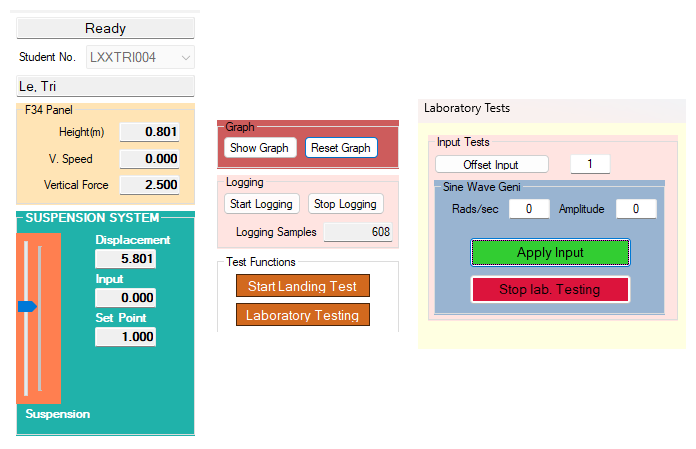
\includegraphics[width=0.92\textwidth]{figures/sim_bench.png}
    \caption{The simulator configured for the step test. The plant is keyed to the student
             number in the top field, so the left column both identifies which plant was
             loaded and reads the $5.801$~m the suspension settled at. On the right,
             \textbf{Offset Input} is $1$ with both sine fields at zero, which is how the
             $1$~V step is applied. The sinusoid runs use the same dialog with
             \textbf{Offset Input} returned to zero and the frequency and amplitude entered
             instead. \textbf{Start Logging} in the middle column opens the CSV and
             \textbf{Logging Samples} counts what has been written to it.}
    \label{fig:bench}
\end{figure}

Two sources of uncertainty need stating before any numbers appear. The logger writes
displacement to $0.001$~m, so any single reading is only known to $\pm 0.5$~mm, and that is the
limit on everything read off the step response. The 100~ms sample period is the other
candidate. A true peak falling between samples reads low and would bias $\zeta$ high. That
effect turns out to be small. Evaluating the identified model at the peak and half a sample
past it puts the worst case at $0.1$~mm, a tenth of a resolution step. The damped period is
$7.4$~s, so $100$~ms is $1.4$\% of it. Quantisation dominates and sampling does not, so the
resolution is the limitation this report carries forward.

One convention follows from the setup rather than from any uncertainty. The step is applied
on top of a non-zero resting displacement, so every amplitude quoted here is a change from
the pre-step baseline, not an absolute displacement.

\section{System Identification}\label{sec:system_id}

\subsection{Step Response Test}\label{sec:step}

A $1$~V step was applied at $t = 9.5$~s and held for the rest of the record.
Figure~\ref{fig:step} is the displacement it produced. The four features marked on it, the
final value, the height of the first peak, the time at which it occurs and the depth of the
undershoot that follows, are the only measurements the step stage needs. Each one is used in
a separate calculation below.

\begin{figure}[h!] \centering 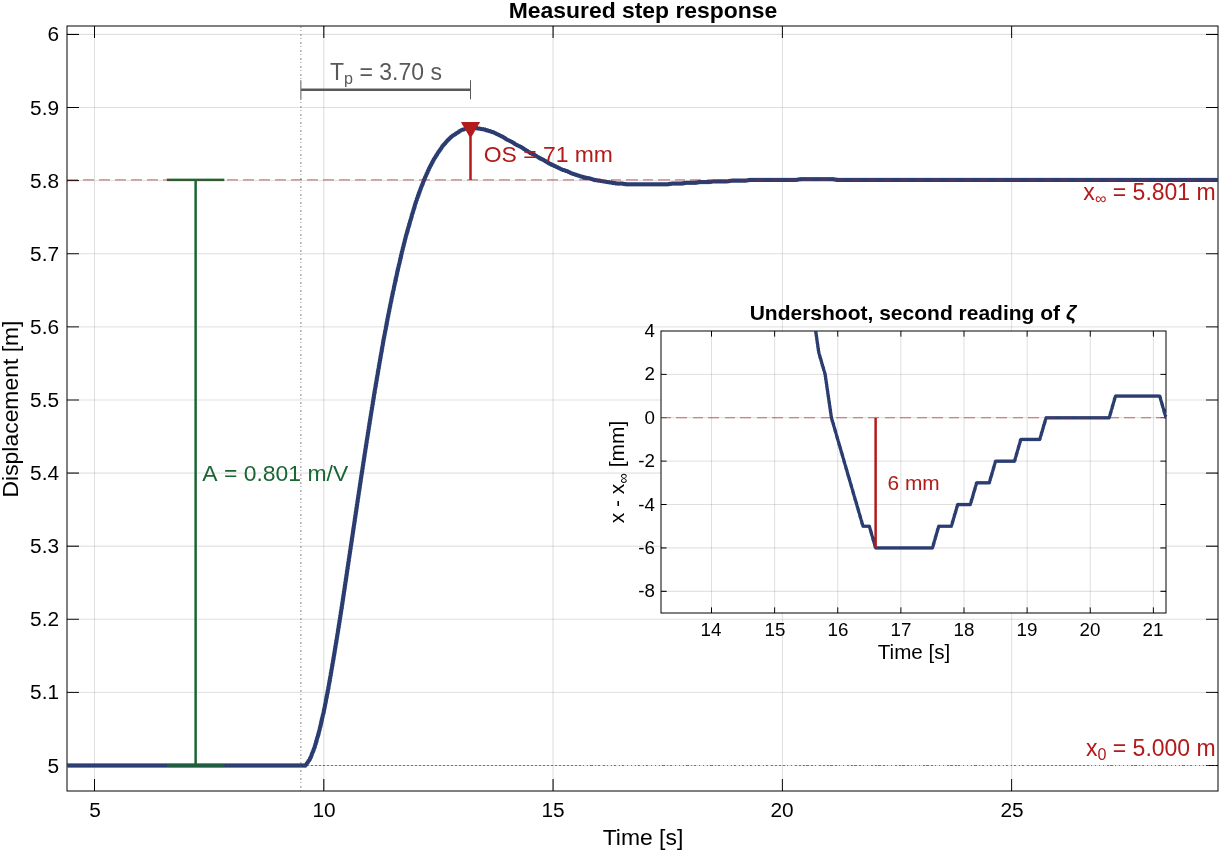
\includegraphics[width=0.8\textwidth]{figures/step_response.png}
\caption{Measured step response, with the four features the analysis reads marked on the graph.
The dotted vertical line is the step. $x_0$ is the pre-step baseline at $5.000$~m and
$x_\infty$ the $5.801$~m the response settles at, so the gap between the two is the rise, $A =
0.801$~m/V. \textbf{OS} marks the first peak, an overshoot of $0.071$~m above the final value,
and $T_p$ the $3.7$~s it takes to get there. The undershoot that follows is $6$~mm on a $0.9$~m
axis, too small to read off the main trace, so it is drawn in the inset against the settled
value. That $6$~mm is six steps of the $0.001$~m logger resolution, and its depth relative to
the first peak gives the second reading of $\zeta$. The staircase in the inset is that resolution made
visible. The second overshoot is predicted at $0.56$~mm and shows up as the single $1$~mm step
near $20.6$~s, the right size for a rounded half step but too coarse to measure, so the damped
period is taken as $T_d = 2T_p$ and not from the spacing of successive peaks.}
\label{fig:step} \end{figure}

\subsubsection*{Question 1. What is the gain of the system?}

Setting $s = 0$ in Equation~\ref{eqn:canonical} leaves $G(0) = A\omega_n^2/\omega_n^2 = A$, so
a step of size $U$ settles at $x_\infty = AU$ above where it started. The gain is therefore
the change in displacement divided by the size of the step,

\begin{equation}\label{eqn:gain}
    A = \frac{x_\infty - x_0}{U} = \frac{5.801 - 5.000}{1} = 0.801~\text{m/V}.
\end{equation}

The baseline $x_0$ is subtracted because the suspension rests at a non-zero displacement
before the step, visible on the left of Figure~\ref{fig:step}. The input value used is the
one recorded in the log, not the number typed into the simulator, in case the
simulator scales it. Equation~\ref{eqn:identities} gives $A = \alpha/k$, so this measurement
alone fixes only the ratio $k/\alpha = 1/A = 1.248$. Separating the two needs $\omega_n$,
which Question~3 supplies from the timing of the response, not its amplitude.

\subsubsection*{Question 2. Does the system have real or complex poles?}

The response in Figure~\ref{fig:step} oscillates about its final value, so the system is
underdamped with $\zeta < 1$ and the poles are therefore a complex conjugate pair. Oscillation
about the final value is only possible when the poles have a non-zero imaginary part, so this
reads straight off the shape of the curve.

Reading it off the shape is an eye judgement, so it was checked by fitting the other case to
the same record. Two real poles put a constant and two decaying exponentials in the partial
fraction expansion, and the Laplace table on the course sheet inverts those three terms to a
step response of the form $c + Pe^{-at} + Qe^{-bt}$. The best such fit, searched over both
rates, lands
$22.2$~mm RMS from the measurement against $5.6$~mm for the complex pair. More telling than
the RMS is what the fit cannot do at all. The measured peak stands $71.0$~mm above the final
value, and a sum of decaying real exponentials never rises above the value it settles to,
so the real fit clears it by nothing. Two real poles cannot produce an overshoot, which
means the single overshoot in Figure~\ref{fig:step} rules them out on its own.

\subsubsection*{Question 3. Where are the dominant poles?}

For an underdamped second order system the fractional overshoot $M_p$ measured from
Figure~\ref{fig:step} fixes the damping ratio,

\begin{equation}\label{eqn:zeta}
    M_p = e^{-\pi\zeta/\sqrt{1-\zeta^2}}
    \quad\Longrightarrow\quad
    \zeta = \frac{-\ln M_p}{\sqrt{\pi^2 + \ln^2 M_p}} = 0.611,
\end{equation}

with $M_p = 0.071/0.801 = 0.0886$ read off Figure~\ref{fig:step}. The second form is the
sheet's overshoot formula solved for $\zeta$. Taking the log of both sides and squaring
turns it into a linear equation in $\zeta^2$. The time to the first peak
is half a damped period, so it fixes the damped natural frequency,

\begin{equation}\label{eqn:wd}
    \omega_d = \frac{\pi}{T_p} = \frac{\pi}{3.7} = 0.849~\text{rad/s},
    \qquad
    \omega_n = \frac{\omega_d}{\sqrt{1-\zeta^2}} = 1.072~\text{rad/s}.
\end{equation}

The poles are the roots of the denominator of Equation~\ref{eqn:canonical}. Completing the
square on $s^2 + 2\zeta\omega_n s + \omega_n^2$ gives
$(s + \zeta\omega_n)^2 + \omega_n^2(1 - \zeta^2)$, and the second term is $\omega_d^2$ by the
$\omega_d = \omega_n\sqrt{1-\zeta^2}$ on the course sheet, so

\begin{equation}\label{eqn:poles}
    s_{1,2} = -\zeta\omega_n \pm j\omega_d = -0.655 \pm j\,0.849.
\end{equation}

How much of the rest of the record is usable follows from where the extrema sit. The course
sheet gives the first one only, at $t_p = \pi/\omega_d$ and $y_p = A(1 + M_p)$, so the rest are
worked out here. The class notes describe the underdamped response as a decaying sinusoid about
the final value, with the decay set by the real part of the poles and so carried by
$e^{-\zeta\omega_n t}$. Its turning points are therefore half a damped period apart, at
$t = n\pi/\omega_d$, and they alternate maximum, minimum, maximum, since consecutive turning
points of a sinusoid fall on opposite sides of the value it oscillates about. Between one and
the next the envelope falls by

\begin{equation}\label{eqn:decayfactor}
    e^{-\zeta\omega_n \pi/\omega_d} = e^{-\zeta\pi/\sqrt{1-\zeta^2}} = M_p,
\end{equation}

where the middle step uses $\omega_d = \omega_n\sqrt{1-\zeta^2}$ from the sheet, and the result
is the same $M_p$ the sheet gives for the overshoot. Applying that factor once per turning
point,

\begin{equation}\label{eqn:extrema}
    x(n\pi/\omega_d) - x(\infty) = (-1)^{n+1} M_p^{\,n} \, \Delta x,
    \qquad n = 1, 2, 3, \dots
\end{equation}

Setting $n = 1$ puts the first extremum at $\Delta x(1 + M_p)$ above the baseline, which is the
$y_p$ the sheet gives, so the general form reduces to the course result in the one case the
course states.

With $M_p = 0.0886$ and a rise of $\Delta x = 0.801$~m that gives $71.0$~mm for the first
overshoot, $6.3$~mm for the undershoot that follows it, and $0.56$~mm for the second
overshoot. The logger resolves $1$~mm, so the first two stand $71$ and $6$ resolution steps
clear of the final value while the third, at half a step, is visible but not measurable. The
logger rounds, so a $0.56$~mm deviation reads as a single $1$~mm step, and the record holds
one from $20.4$ to $21.1$~s against a predicted $20.6$~s. Its timing corroborates
Equation~\ref{eqn:extrema}, but one step could be anything from $0.5$ to $1.5$~mm, so it
carries no usable amplitude. Two extrema are therefore usable, not three.

The undershoot is in the record. The output holds at $5.795$~m from $16.6$ to $17.5$~s,
$6$~mm below the final value, against the $6.29$~mm at $16.9$~s that
Equation~\ref{eqn:extrema} predicts. Its timing is not usable, because quantisation flattens
the bottom of the trough across nearly a second, which is why the damped period above is
still taken from the sharp first peak. Its amplitude is usable, and the ratio of the two
deviations is a second reading of the damping ratio,

\begin{equation}\label{eqn:logdec}
    \frac{|x_2 - x(\infty)|}{|x_1 - x(\infty)|} = \frac{6}{71} = 0.0845
    \quad\Longrightarrow\quad
    \zeta = \frac{-\ln 0.0845}{\sqrt{\pi^2 + \ln^2 0.0845}} = 0.618,
\end{equation}

against $0.611$ from the overshoot. Carrying the $\pm 0.5$~mm resolution on the $6$~mm
reading through Equation~\ref{eqn:logdec} puts this second $\zeta$ between $0.606$ and
$0.631$, a band that contains the overshoot value.

Two readings of the same quantity are worth more than the sum of their parts here, because the
peak enters the two calculations in opposite senses. In Equation~\ref{eqn:zeta} the peak height
is the numerator, so reading it too high lowers $\zeta$; in Equation~\ref{eqn:logdec} it is the
denominator, so reading it too high raises $\zeta$. A misread peak therefore does not shift
both answers together, it pulls them apart. Reading $75$~mm instead of $71$~mm would put them
at $0.602$ and $0.627$, a gap of $0.025$ against the $0.007$ actually obtained. The two
agreeing to within a third of the resolution band is what makes the $71$~mm reading itself
trustworthy, and the damping ratio with it. Section~\ref{sec:freq} adds a third reading from
the resonant peak, a stronger check again because it comes from a different experiment and uses
none of the step record.

\subsubsection*{Question 4. What corner frequency follows from that?}

For a second order system with no zeros the magnitude asymptotes cross at the undamped
natural frequency, so the expected corner frequency is $\omega_n = 1.072$~rad/s. This is
a prediction made from the step data alone, and it is what the frequency response test in
Section~\ref{sec:freq} is used to confirm.

\subsection{Frequency Response}\label{sec:freq}

The simulator applies one sinusoid at a time instead of sweeping, so the frequencies have to be
chosen in advance. They are placed around the corner frequency predicted in Question~4, since
that is where the magnitude peak and the $-90^\circ$ phase crossing sit and where the curve
carries the most information about $\zeta$. Two points well below and two well above $\omega_n$
fix the low frequency gain and the high frequency roll-off. Together they confirm the system is
second order rather than first.

\begin{table}[h!]
\centering
\begin{tabular}{lrrrr}
\toprule
\textbf{Point} & \textbf{$\omega$ [rad/s]} & \textbf{Amplitude ratio} &
\textbf{$|G|$ [dB]} & \textbf{Phase [deg]} \\
\midrule
$0.14\,\omega_n$ & 0.15 & 0.805 & $-1.89$ & $-10.8$ \\
$0.28\,\omega_n$ & 0.30 & 0.815 & $-1.78$ & $-22.2$ \\
$0.47\,\omega_n$ & 0.50 & 0.827 & $-1.65$ & $-39.2$ \\
$0.75\,\omega_n$ & 0.80 & 0.789 & $-2.06$ & $-69.1$ \\
$0.93\,\omega_n$ & 1.00 & 0.696 & $-3.15$ & $-89.7$ \\
$1.21\,\omega_n$ & 1.30 & 0.512 & $-5.81$ & $-115.5$ \\
$1.87\,\omega_n$ & 2.00 & 0.236 & $-12.53$ & $-149.2$ \\
$2.80\,\omega_n$ & 3.00 & 0.105 & $-19.60$ & $-170.9$ \\
$3.73\,\omega_n$ & 4.00 & 0.059 & $-24.63$ & $-183.8$ \\
$5.60\,\omega_n$ & 6.00 & 0.026 & $-31.60$ & $-202.1$ \\
$7.46\,\omega_n$ & 8.00 & 0.015 & $-36.43$ & $-216.8$ \\
$9.33\,\omega_n$ & 10.00 & 0.010 & $-39.99$ & $-230.1$ \\
\bottomrule
\end{tabular}
\caption{Frequency response measurements. Amplitude ratio and phase are fitted by least
squares at the known drive frequency, over the part of each log after the transient has
decayed. The round values in the second column are the frequencies actually set at the bench,
chosen around the corner frequency Question~4 predicts. The first column divides each of them
by that $\omega_n = 1.072$~rad/s, so the table can be read against the corner directly.}
\label{tab:freq}
\end{table}

The gain can be read a second time here, from the flat low frequency end of
Figure~\ref{fig:bode}, where $|G| \to A$. That gives $A = 0.805$ m/V against $0.801$ m/V
from the final value of the step, a difference of $0.5$\%.

The whole of that difference is accounted for. The low frequency end of a Bode plot is only
flat in the limit, and the lowest frequency tested sits at $0.14\,\omega_n$, far enough up
the curve that the magnitude has already begun to rise towards resonance. Putting $s = j\omega$
into Equation~\ref{eqn:canonical}, taking the magnitude and dividing numerator and
denominator by $\omega_n^2$ gives

\begin{equation}\label{eqn:maglift}
    \frac{|G(j\omega)|}{A} =
    \frac{1}{\sqrt{\left(1 - (\omega/\omega_n)^2\right)^2 + \left(2\zeta\omega/\omega_n\right)^2}}
\end{equation}

Evaluated at the three lowest frequencies this is the lift over the true DC gain, and
dividing it out of each measurement recovers what each run would have read at zero
frequency.

\begin{center}
\begin{tabular}{cccc}
\toprule
$\omega$ [rad/s] & lift over DC & measured $|G|$ & implied $A$ \\
\midrule
$0.15$ & $+0.48$\% & $0.8049$ & $0.8010$ \\
$0.30$ & $+1.73$\% & $0.8149$ & $0.8010$ \\
$0.50$ & $+3.32$\% & $0.8274$ & $0.8008$ \\
\bottomrule
\end{tabular}
\end{center}

against $0.8010$ m/V from the step. Three sine runs and one step run agree on the gain to
$0.03$\%, and the $0.5$\% that looked like disagreement was the plateau being read at
$0.15$ rad/s and treated as though it were at zero.

This beats the two damping readings of Section~\ref{sec:step}, because those both came out of
\texttt{step1.csv} and shared the peak measurement between them. These share almost nothing. The
step gain is read from the settled value of one record, and the frequency gain from
sinusoidal fits to three separate records taken at different times. The one thing they do share
is that the lift divided out above is computed from the step $\zeta$ and $\omega_n$, and that
dependence is weak enough to ignore. Repeating the correction with $\zeta = 0.620$ instead of
$0.611$ moves the lift at $0.15$~rad/s from $0.48$\% to $0.44$\%, or $0.04$\% on $A$, a tenth
of the agreement being claimed. So their agreement fixes $A$ independently for practical
purposes, and any disagreement found later in this report has to be explained somewhere other
than the gain.

Figure~\ref{fig:bode} plots those points against the response of the model identified from
the step test. The magnitude peak sits at $0.50$ rad/s and the phase
passes $-90^\circ$ at $1.003$ rad/s, against the $\omega_n = 1.072$
rad/s predicted in Question~4, a difference of $6.5$\%.

That confirms the step estimate instead of contradicting it, because the crossing is not
expected to land on $\omega_n$ in the first place. Only a system with nothing but the two
poles passes $-90^\circ$ exactly at $\omega_n$, and Section~\ref{sec:validation} identifies a
$101$~ms transport delay in this measurement chain. A delay subtracts phase in proportion to
frequency, so it pushes the phase curve down everywhere, and a curve pushed down everywhere
reaches $-90^\circ$ sooner, at a lower frequency. Adding the delay to the identified model
moves its crossing from $1.072$ to $1.007$~rad/s, $6.1$ of the $6.5$\% observed.
The $0.4$\% left over is smaller than the gap between the measured points at $1.00$ and
$1.30$~rad/s that the crossing is interpolated from, so nothing in the phase data asks for a
different $\omega_n$ than the step test gave.

\begin{figure}[h!] \centering 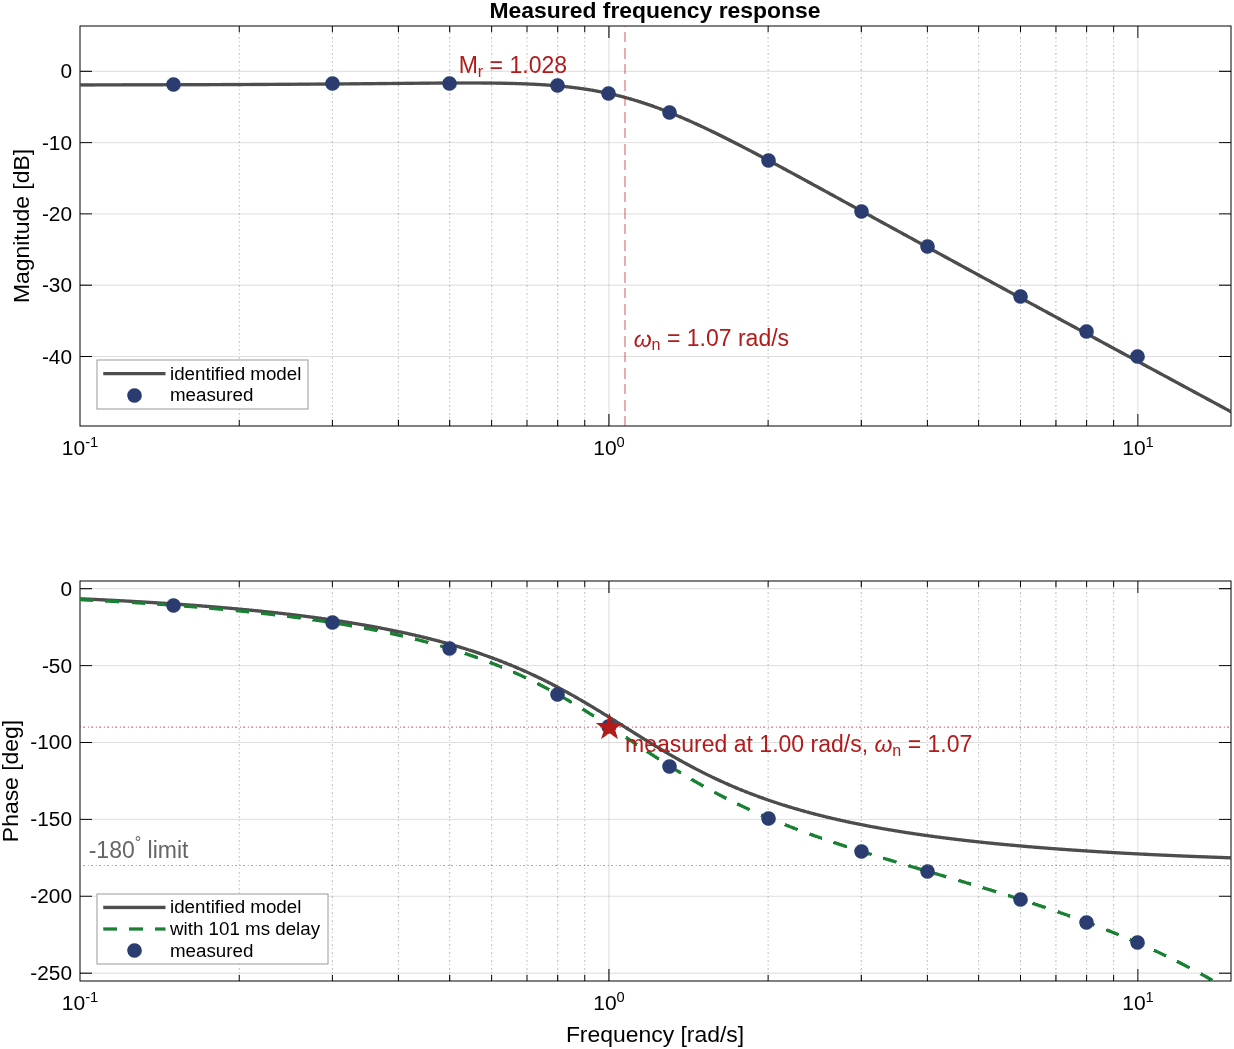
\includegraphics[width=0.8\textwidth]{figures/bode_plot.png}
\caption{Measured frequency response against the model identified from the step test, with the
features used below marked on both panels. The dashed line at $\omega_n$ is the $1.072$~rad/s
the step data gives. The measured phase crosses the marked $-90^\circ$ at $1.003$~rad/s, marked
with a star, and that gap of $0.07$~rad/s is the first sign of the delay
Section~\ref{sec:validation} identifies. $M_r$ is the magnitude peak, at $0.50$~rad/s and a
height of $0.827$~m/V, which is $1.028$ times the lowest measured point. Both the frequency and
the height are predicted by the step parameters alone. The measured phase runs past the marked
$-180^\circ$ limit, which no second order system can do, and that is what identifies the delay.
The flat low frequency end of the magnitude panel is where the frequency test reads the gain a
second time. The lowest point sits at $0.805$~m/V, which the text corrects to $0.801$ for the
residual rise toward resonance.} \label{fig:bode} \end{figure}

The height of the magnitude peak is a third reading of the damping ratio, and the first
taken from a different experiment. This one is not on the course sheet, so it is obtained here
by maximising Equation~\ref{eqn:maglift} over $\omega$, which is itself just the sheet's
canonical form evaluated at $s = j\omega$. Writing $u = \omega/\omega_n$, the bracket under
the square root is $(1-u^2)^2 + (2\zeta u)^2$, a quadratic in $u^2$ with its minimum at
$u^2 = 1 - 2\zeta^2$. That minimum only exists for $\zeta < 1/\sqrt{2}$, and it puts the
peak at $\omega_r = \omega_n\sqrt{1 - 2\zeta^2}$; substituting it back gives the height

\begin{equation}\label{eqn:mr}
    M_r = \frac{1}{2\zeta\sqrt{1-\zeta^2}},
\end{equation}

Which gain the peak is measured against decides how independent the answer is, and the two
choices available here pull in opposite directions. Dividing by the lowest point swept uses
nothing but sine data, and gives $M_r = 1.028$ and $\zeta = 0.620$. Dividing by the
$0.8010$~m/V reconstructed above is the more accurate of the two, since
Equation~\ref{eqn:maglift} has already shown the lowest point to sit $0.48$\% above DC, and
gives $M_r = 1.033$ and $\zeta = 0.612$. But that reconstruction takes $\zeta$ and
$\omega_n$ as inputs, and the only values available at this stage are the step ones, so the
corrected reading is not independent of the test it is being compared against.

The honest independent number is therefore $\zeta = 0.620$, which sits $1.5$\% above the
$0.611$ from the overshoot and $0.3$\% above the $0.618$ from the decay ratio in
Equation~\ref{eqn:logdec}. The gap to the corrected reading is accounted for and is not
scatter: $M_r$ moves by the $0.48$\% bias in the reference gain, and Equation~\ref{eqn:mr}
amplifies that by a factor of about $2.5$ on the way into $\zeta$ because
$\mathrm{d}M_r/\mathrm{d}\zeta$ is shallow here, the $1.3$\% between $0.620$ and $0.612$.
Quoting $0.612$ and calling it agreement to $0.1$\% would be reporting the correction rather
than the measurement.

Putting that $\zeta$ and the frequency the peak was recorded at into $\omega_r$ above recovers
$\omega_n = 1.039$ rad/s, a second reading of that quantity but a far weaker one than the
damping ratio it came from, for two reasons. The peak was recorded at $0.50$ rad/s, but the
sweep only sampled $0.30$, $0.50$ and $0.80$ in that region, so a true peak anywhere between
about $0.40$ and $0.65$ rad/s would have been recorded in the same place, which on its own
spreads $\omega_n$ from $0.83$ to $1.35$ rad/s. On top of that $\sqrt{1-2\zeta^2}$ is only
$0.481$ here, close enough to zero that differentiating it amplifies a relative error in
$\zeta$ roughly threefold on the way into $\omega_n$. The damping ratio survives this equation.
The natural frequency does not, and $\omega_n$ is taken instead from the step timing and from
the least squares fit below.

All three readings of $\zeta$, at $0.611$, $0.618$ and $0.620$, fall inside the $0.606$ to
$0.631$ band that the resolution puts on the decay ratio, and the checks are not
interchangeable. The decay ratio is the narrow one. It shares \texttt{step1.csv} with the
overshoot, but because the peak enters the two formulas in opposite senses, a disagreement
between them points at the peak measurement and nothing else. The resonant peak is the broad
one. It can say nothing about which step measurement failed, but it is the only reading that
could catch a fault in the step record itself, such as a plant that had not fully settled
before the step or a step that was not the $1$~V it was set to. Two readings of one record
agree with each other whether or not that record is sound, so it takes the sine runs to rule
that out. Having both, one damping ratio has been confirmed narrowly within the step test
and broadly against a separate experiment, and $\zeta = 0.611$ is carried forward on that
basis.

Running the comparison the other way is a stronger test still, because it uses none of the
step data. Fitting $A$, $\zeta$, $\omega_n$ and a transport delay to the twelve points of
Table~\ref{tab:freq} by least squares gives $A = 0.814$~m/V, $\zeta = 0.612$,
$\omega_n = 1.067$~rad/s and $T = 101$~ms, against $0.801$, $0.611$ and $1.072$ from the step
test. Magnitude in dB and phase in degrees are weighted equally, since the two residuals
scatter by about the same amount on this data, $0.24$~dB against $0.2^\circ$. The two
experiments share no measurement, and their damping ratios agree to $0.1$\% and their natural
frequencies to $0.5$\%.

The gain is the one parameter this fit reads worse than the reconstruction of
Equation~\ref{eqn:maglift}, and the reason for that belongs in the report, not a quiet pick of
whichever number flatters the model. The magnitude residuals are not scattered about zero, they
slope. The fit sits above every measured point below $6$~rad/s, by $+0.14$~dB at the bottom of
the sweep, and falls to $-0.63$~dB at $10$~rad/s. The tail discussed below, $-39.1$ against
$-40$~dB/decade, is what does it, and least squares answers by lifting the whole magnitude
curve until the tail error is shared out, $1.7$\% of gain. Refitting the seven points at or
below $2$~rad/s returns $A = 0.802$~m/V, within $0.1$\% of the step, leaves
$\omega_n = 1.067$~rad/s untouched and moves $\zeta$ only in the fourth decimal, from
$0.6115$ to $0.6114$. The shape parameters are
therefore genuinely independent of which points are used. Only the gain is sensitive, and it is
taken from the low frequency points where it is the only thing being measured.

The high frequency slope, fitted over the $5$ points above $2\omega_n$, is $-39.1$ dB/decade
against the $-40$~dB/decade expected of a system with two poles and no zeros. That asymptote is
only reached well above the corner, so the comparison is only fair if the fitted points sit far
enough out. Differentiating the identified model shows they do. Its local slope is only $-20.0$
dB/decade at $\omega_n$ itself, steepens to $-36.5$ by $1.5\,\omega_n$, and reaches $-40.0$ at
$2\omega_n$, the first point in the fit. It runs between $-40.0$ and $-40.7$ across the whole
fitted range and is back at $-40.1$ by the highest frequency tested, $9.33\,\omega_n$. Note
that the approach is from above rather than below. At $\zeta = 0.611$ there is no sharp
resonance for the curve to fall off, so it eases down onto the asymptote instead of diving past
it.

Fitting the model over those same five points gives $-40.4$ dB/decade against the measured
$-39.1$. The $1.3$ dB/decade between them is $0.68$~dB across the $0.52$ decades from $3$ to
$10$~rad/s, roughly two to three times the $0.24$~dB RMS scatter of the magnitude fit, and
in the direction expected as the signal shrinks. At $10$~rad/s the output amplitude is
$0.0100$~m, ten steps of the logger resolution.

The slope therefore supports the second order model instead of merely reflecting where the
points sit, and the margin is not close. Each additional pole adds $-20$~dB/decade, so a
three pole system would roll off near $-60$. The measurement is $2.3$\% away from two poles
and $35$\% away from three. No second corner appears anywhere in Figure~\ref{fig:bode}
either. The magnitude runs straight from $2$ to $10$~rad/s with no second break in it, and a
non-dominant pole inside the tested band would have shown as one. Any pole this test cannot
see must sit above $10$~rad/s, more than nine times $\omega_n$ and far too fast to matter to
the dominant response.

\subsection{Identified Model}

\begin{table}[h!] \centering \begin{tabular}{lrp{6.2cm}} \toprule \textbf{Quantity} &
\textbf{Value} & \textbf{Source} \\ \midrule Gain $A$ & $0.801$ m/V & Equation~\ref{eqn:gain},
final value of Figure~\ref{fig:step} \\ Damping ratio $\zeta$ & $0.611$ &
Equation~\ref{eqn:zeta}, overshoot of Figure~\ref{fig:step} \\ Natural frequency $\omega_n$ &
$1.072$ rad/s & Equation~\ref{eqn:wd}, time to first peak, confirmed in Figure~\ref{fig:bode}
\\ Spring coefficient $k$ & $1.150$ s$^{-2}$ & $k = \omega_n^2$ \\ Damping coefficient $b$ &
$1.310$ s$^{-1}$ & $b = 2\zeta\omega_n$ \\ Input scaling $\alpha$ & $0.921$ m\,V$^{-1}$s$^{-2}$
& $\alpha = Ak$ \\ Poles & $-0.655 \pm j0.849$ & Equation~\ref{eqn:poles} \\ Delay $T$ &
$0.101$ s & Section~\ref{sec:validation}, phase residual \\ \bottomrule \end{tabular}
\caption{Identified parameters of the suspension. Everything is scaled to the mass, as
Equation~\ref{eqn:eom} sets out, so $k$ carries stiffness per unit mass and $b$ damping per
unit mass, which is why their units are powers of seconds and not N\,m$^{-1}$ and
N\,s\,m$^{-1}$.} \label{tab:model} \end{table}

Substituting Table~\ref{tab:model} into Equation~\ref{eqn:tf_input}, the identified plant is

\begin{equation}\label{eqn:identified}
    G(s) = \frac{0.921}{s^2 + 1.310\,s + 1.150}.
\end{equation}

Had $\alpha$ been assumed equal to $1$, Equation~\ref{eqn:identities} would give $k$ twice
over, once as $1/A = 1.248$ from the steady state gain and once as $\omega_n^2 = 1.150$ from
the oscillation. Those differ by $8.6$\%, and the size of that gap is what rules the assumption
out. The sampling limits are an order of magnitude too small to produce it. Closing it through
$T_p$ would need $3.55$~s against the $3.7$~s measured, one and a half sample periods, and
closing it through the overshoot would need $0.055$~m against the $0.071$~m measured, sixteen
times the logger resolution. Neither error is available. The first would need the peak to have
been mistimed by one and a half samples in a record where the peak is $71$ resolution steps
tall and the sampling error is a tenth of one step, and the second would need an overshoot
reading wrong by sixteen steps. The measurements are not what is wrong. The assumption is. The
input is scaled, and

\begin{equation}\label{eqn:alpha}
    \alpha = Ak = 0.801 \times 1.150 = 0.921,
\end{equation}

so the logged input column is not the force in the units Equation~\ref{eqn:eom} assumes but
about $92$\% of it. The least squares fit to the seven frequency points at or below $2$~rad/s
settles the question, since it uses no step data at all. It returns $A = 0.802$~m/V and
$\omega_n = 1.067$~rad/s, hence $\alpha = 0.913$. Two experiments that share no measurement put
$\alpha$ at $0.921$ and $0.913$, and neither puts it at $1$, which is what makes this a
property of the simulator, not an artefact of how the step was read.

The two coefficients come from different measurements, so they fail differently. $k$ rests on
$\omega_n$, which comes from the timing of the first peak and is confirmed to $0.5$\% by the
frequency fit. $b$ rests on $\zeta$, which comes from the height of that peak, is confirmed
to about $1$\% by the decay ratio and the resonant peak, but carries the wider band because
the $6$~mm undershoot it is checked against is only six resolution steps deep.
Of the two, $k$ is the one to trust. Carrying those bands through $k = \omega_n^2$ and $b =
2\zeta\omega_n$ puts $k$ inside about $1$\% and $b$ inside about $1.7$\%, since $b$ inherits
the error on $\omega_n$ on top of the wider one on $\zeta$. Where the two would place the poles
differently, the timing measurement is the one to follow.

\subsection{Model Validation}\label{sec:validation}

Equation~\ref{eqn:identified} was simulated and overlaid on the measurements it was built
from. Figure~\ref{fig:validation} shows the comparison for the step test, with an RMS error
of $0.0056$ m over the logged response, $0.7$\% of the $0.801$~m rise.
Figure~\ref{fig:validation_freq} is the same test in the frequency domain. Both use a model
drawn from the step parameters only, so any agreement with the measured points is genuine
confirmation and not a fit.

\begin{figure}[h!] \centering
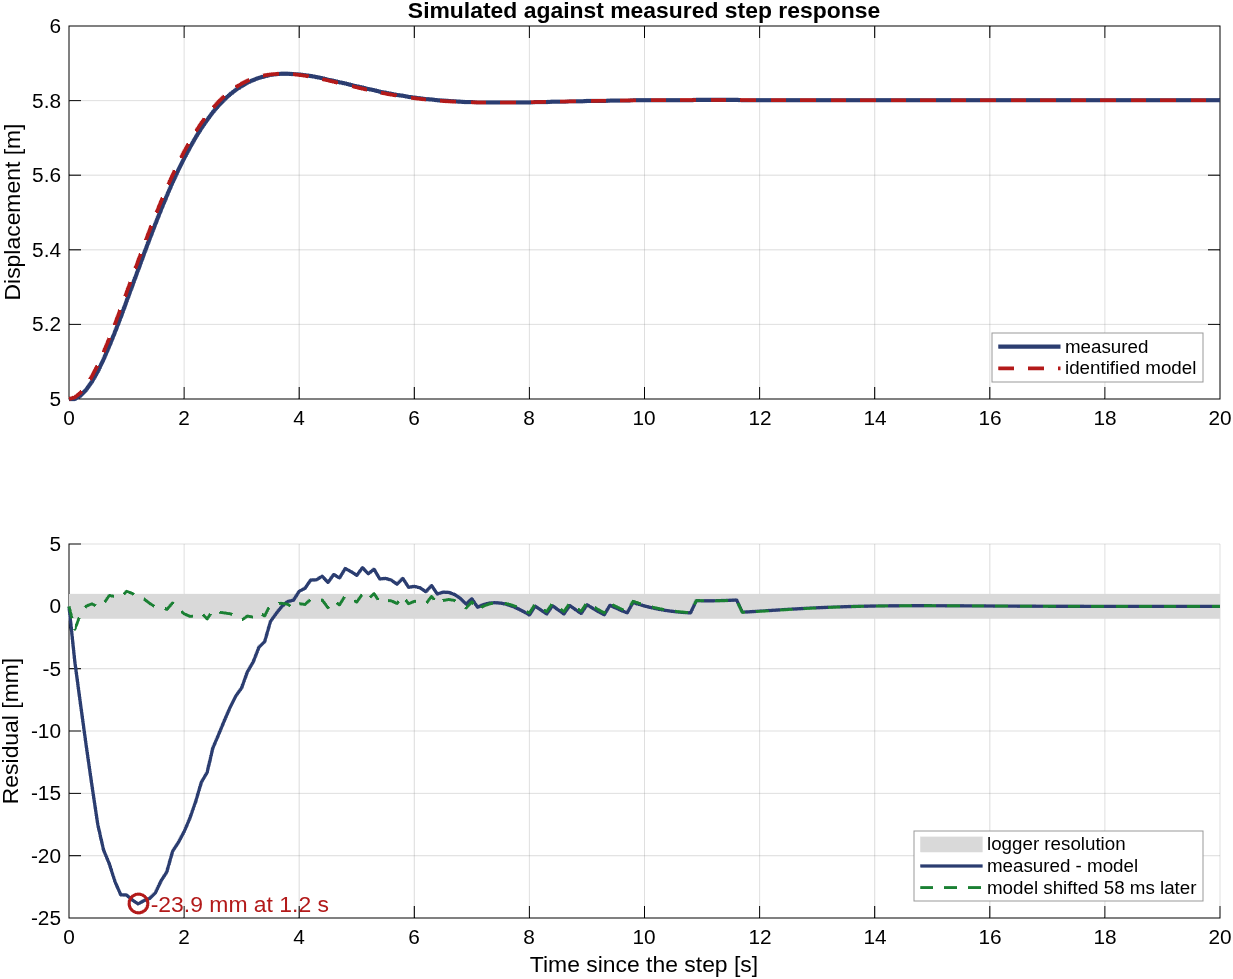
\includegraphics[width=0.8\textwidth]{figures/validation_step.png} \caption{Simulated response
of the identified model against the measured step response, with the residual below. The two
curves are a line width apart on the displacement axis, so the lower panel plots their
difference in millimetres against the shaded $\pm 1$~mm the logger can resolve. The RMS error
over the whole record is $0.0056$~m. It is not spread across the record. The residual reaches
$-23.9$~mm at $1.2$~s, is back inside the logger resolution from $6.7$~s on, and the
measurement sits below the model throughout the rise. The dashed trace is the same residual
after the model is shifted $58$~ms later. That shift is the best pure one available, and it
leaves almost nothing outside the resolution band.} \label{fig:validation} \end{figure}

The lower panel of Figure~\ref{fig:validation} says where. Not on the final value, which agrees
to better than the logger resolution from $6.7$~s on, and not on the height of the first peak,
which the model reproduces. The disagreement is all on the rising edge. The measurement sits
$23.9$~mm below the model at $1.2$~s, crosses back through zero at $3.7$~s where the peak is,
overshoots to at most $3.1$~mm the other way and then stays inside the $\pm 1$~mm band. That is
the shape of a model running early, not of one with the wrong gain or the wrong damping, and
shifting it $58$~ms later with no parameter touched takes the RMS error from $5.6$~mm to
$0.32$~mm and the worst single sample from $23.9$~mm to $1.9$~mm.

Of the assumptions in Section~\ref{sec:modelling} it points at one only. Equation~\ref{eqn:eom}
has the force reaching the mass at the instant the input column records it, and that is what a
residual removable by a pure time shift contradicts. Linearity, the second order structure and
the mass normalisation survive it untouched, since none of them can be repaired by moving the
model along the time axis, and the amplitude repeats below test linearity on its own. The model is good enough to design a controller against. The gain
and the pole locations are within about $1$\% and the delay is small against the $7.4$~s damped
period, but it has to be carried rather than dropped, because it is phase margin the controller
does not get back.

That figure plots the residual point by point, which is what Figure~\ref{fig:bode} cannot show
at the scale it is drawn at. Quantified over the points of Table~\ref{tab:freq}, the model
predicts the measured magnitude to $0.24$ dB RMS and the measured phase to $25.5$ degrees RMS.
Reporting both domains matters because they fail differently. A magnitude error that is uniform
across frequency is a gain or scaling problem, while an error that grows with frequency points
at the damping term instead. The errors here follow neither pattern cleanly, and that is the
useful part. The magnitude residual is not uniform and not growing in any way that implicates
the damping. It sits below $0.06$~dB at every point up to $3$~rad/s, a quarter of the
resolution of the fit. It lifts only at $6$, $8$ and $10$~rad/s, to $+0.17$, $+0.37$ and
$+0.70$~dB, and there the output amplitude has fallen to $26$, $15$ and $10$ steps of the
logger resolution. What that shows is the measurement running out of signal at the top of the
sweep, not the model failing. Across the band where the signal is strong the magnitude is
essentially exact.

\begin{figure}[h!] \centering
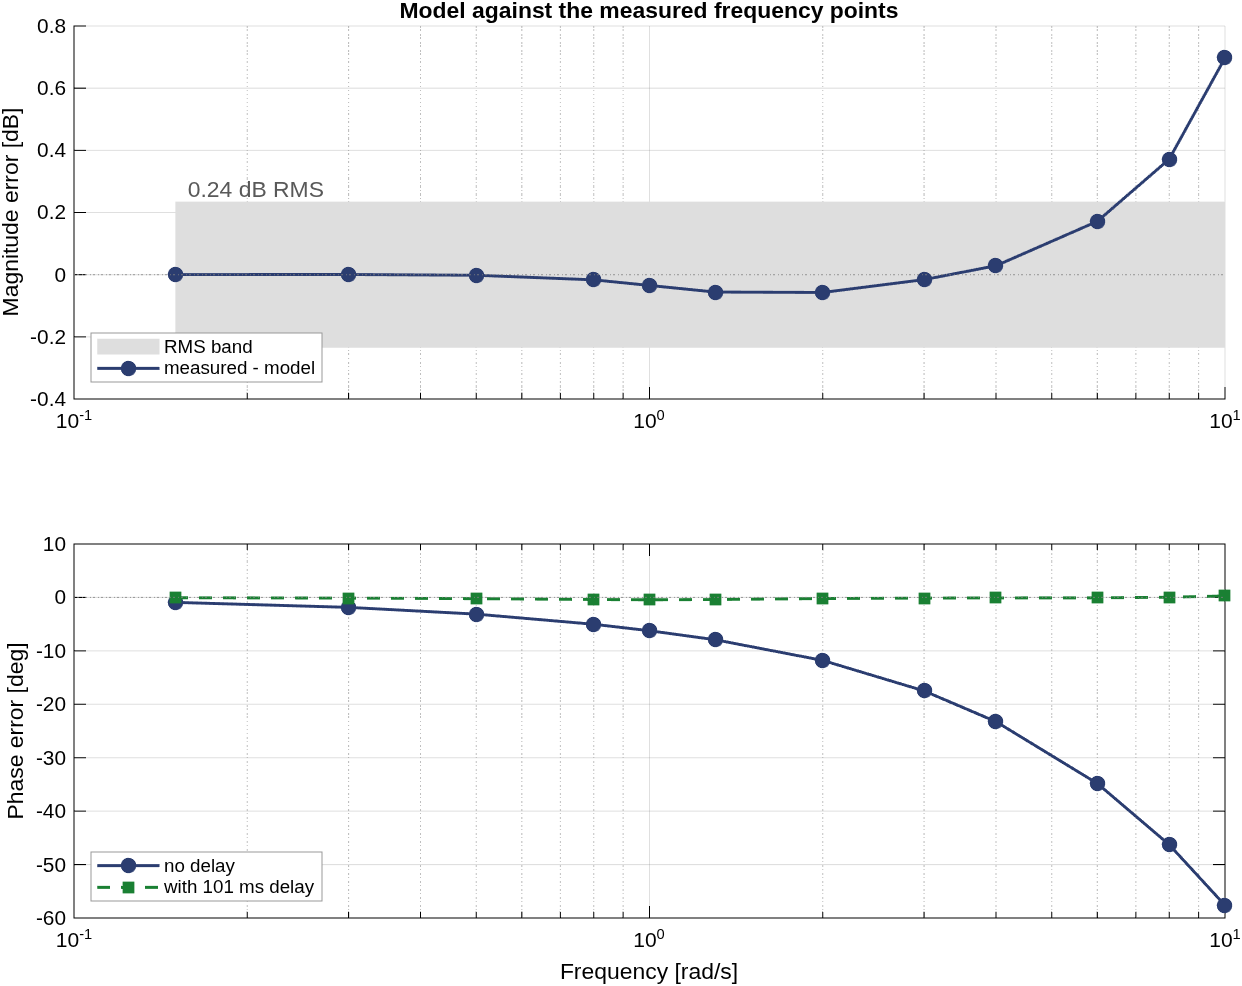
\includegraphics[width=0.8\textwidth]{figures/validation_freq.png} \caption{Identified model
against the measured frequency points, plotted as the residual instead of as two curves. The
magnitude error, above, stays inside the $0.24$~dB RMS band until $6$~rad/s and then lifts, at
exactly the points where the output amplitude has fallen to a few resolution steps. The phase
error, below, does not scatter. It follows $-\omega T$ with $T = 101$~ms across two decades,
which is a delay and not a missing pole. Including it leaves the squares, $0.2^\circ$ RMS with
no point worse than $0.45^\circ$.} \label{fig:validation_freq} \end{figure}

The phase residual behaves completely differently. It grows steadily and without turning
over, from $-0.9^\circ$ at $0.15$~rad/s to $-57.6^\circ$ at $10$~rad/s, and it does so at
frequencies where the magnitude is still being predicted to hundredths of a decibel. So the
two do not fail together. Whatever is missing from Equation~\ref{eqn:identified} changes
phase while leaving gain alone, which rules out every explanation that would move both.
A wrong gain, a wrong damping ratio, a wrong natural frequency, or a missing pole would all
show in the magnitude first.

The phase disagreement is not a small residual. The measured phase passes $-180^\circ$ and
reaches $-230^\circ$ at the highest frequency tested, and no second order system can exceed
$-180^\circ$ at any frequency. Something outside Equation~\ref{eqn:identified} is therefore
present. Subtracting the model phase from the measurement leaves an excess that grows close to
linearly with $\omega$, which is the signature of a pure time delay rather than of an
additional pole. A pole contributes a lag that saturates, while a delay contributes $-\omega T$
without bound and leaves the magnitude untouched, since holding a sinusoid back by $T$ seconds
shifts it by $\omega T$ radians and changes its amplitude not at all. The delay term $e^{-sT}$ is the one piece of
the final model that is not on the course sheet, and neither is it in the Laplace table there,
since the sheet covers second order systems and this is a property of the measurement chain,
not of the suspension. A least squares fit of that excess gives

\begin{equation}\label{eqn:delay}
    T = 0.101~\text{s},
\end{equation}

against the $0.100$~s sampling period of the logger, an agreement of $1$\%. A lag inside the
suspension would have no reason to equal the logging period. Something in the measurement
chain has every reason to. I therefore treat it as an artefact of that chain and not as part
of the plant, which is why it changes neither $k$ nor $b$ in Table~\ref{tab:model}. It stays
in the model regardless, because a controller reads the plant through the same chain.

The step test does not return the same number, and the difference is larger than it first
looks. The best pure time shift on \texttt{step1.csv} is $58$~ms, and the obvious defence, that
a step can only place the onset to the sample it landed in, does not survive the repeats.
The three runs were triggered at $9.5$, $5.2$ and $4.4$~s. If the onset fell between samples
by a different fraction each time, the best shift would scatter across those runs by up to
half a sample. It does not move at all. All three return $58$~ms, and after the step the three
records are identical sample for sample. The simulator lands the step on a sample boundary
every time, so there is no sub-sample uncertainty to absorb the difference. The step number is
also better determined than one fitted shift suggests, since the samples $0.2$ to $0.5$~s
after the step sit $9$, $25$, $47$ and $74$~mm above the baseline, and the undelayed model
reaches those four heights $55$, $53$, $55$ and $55$~ms earlier.

So the two experiments genuinely disagree, at $58$~ms against $101$~ms, and
Table~\ref{tab:refit} shows the frequency points are not indifferent about it: held at $58$~ms
the phase residual is $9.5^\circ$ RMS against $0.1^\circ$ at $101$~ms. The candidate that fits
both is the zero order hold. The simulator drives the input through a $100$~ms sampled channel,
and what a hold of period $T_s$ makes of each sample is a pulse one period long, a step minus
a step delayed by $T_s$, scaled by $1/T_s$ so DC passes at unit gain. Its transfer function is
therefore $(1 - e^{-sT_s})/(sT_s)$, and at $s = j\omega$ the numerator factors as
$e^{-j\omega T_s/2}$ times $2j\sin(\omega T_s/2)$, which makes the phase exactly
$-\omega T_s/2$ and the magnitude $\mathrm{sinc}(\omega T_s/2)$.
It puts $50$~ms of apparent delay into a sine sweep, where the hold
acts every sample, and none into a step, a single edge the hold passes once. Adding it to a
$58$~ms transport lag gives $108$~ms against the $101$~ms fitted, the right size.

I am not claiming it as settled, because the same hold attenuates as well as delays. Its
sinc term is $-0.36$~dB at $10$~rad/s, and the measured
magnitude there sits $0.70$~dB \emph{above} the model, not below it. The test that would
settle it needs no new data and is set out under improvements at the end of this section.
What can be said now is
that the $101$~ms is what the frequency data requires, the $58$~ms is what the step data
requires, and the gap between them is not measurement resolution.
Equation~\ref{eqn:identified_delay} carries the $101$~ms because the frequency points are the
more sensitive of the two tests to it. Including it,

\begin{equation}\label{eqn:identified_delay}
    G(s) = \frac{0.921\,e^{-0.101s}}{s^2 + 1.310\,s + 1.150},
\end{equation}

reduces the phase error from $25.5^\circ$ RMS to $0.2^\circ$ RMS over the same twelve points,
while leaving the magnitude fit unchanged because a delay has unit magnitude at every
frequency. It also accounts for the $6.5$\% by which the measured $-90^\circ$ crossing sits
below $\omega_n$. The delayed model crosses $-90^\circ$ at $1.007$ rad/s, not at $1.072$ rad/s.

One qualification belongs here. The excess per unit frequency is not perfectly constant, it
rises from $6.18$ degrees per rad/s at the bottom of the sweep to $6.23$ near $\omega_n$ and
then falls to $5.76$ at $10$ rad/s, so the delay is an
approximation rather than an exact description.

It is close enough to treat as one anyway. What is left after the delay is $0.2^\circ$ RMS
across measurements running out to $-230^\circ$, the same order as the $0.24$~dB the magnitude
fit carries, so the residual has fallen to the level of the measurement itself. Anything more
elaborate would be fitting structure this data cannot resolve. The single number also was not
free to be anything. It accounts for $25.3^\circ$ of the $25.5^\circ$ the second order model
could not, and it landed within $1$\% of the logger sample period, a quantity measured
independently of this fit.

\subsubsection*{Repeatability}

The step test was run $3$ times without changing anything, so the spread across those runs
separates the uncertainty of the method from the error of the model. The three records agree
to the resolution of the logger on every feature used, returning the same $A$, $\zeta$ and
$\omega_n$ to every figure quoted. The simulator is deterministic and the repeats mostly
measure that, which is what makes the comparison decisive: Figure~\ref{fig:validation}
carries $0.0056$~m RMS against repeats that differ by nothing at all. Had they scattered by a
few millimetres the model error could have been dismissed as run to run noise. They did not,
so every millimetre of it is the model. The different trigger times of the three runs are
also what carried the sub-sample timing argument made above, where the $58$ against $101$~ms
gap is discussed.

The same result sets the honest precision of this report. The repeats fix nothing about how
many figures to quote, since they have no spread, but the logger resolution does. At
$0.001$~m on a $0.801$~m rise, the gain is known to about $0.1$\% and nothing here should be
quoted past four figures. The parameters in Table~\ref{tab:model} are given to three or four
accordingly.

\subsubsection*{Linearity}

Every equation in this report assumes the plant is linear, and two of the logged runs test that
directly instead of assuming it. The step test was repeated at $2$~V instead of $1$~V. The
displacement changed by $1.602$~m against $0.801$~m, exactly twice, so both records return a
gain of $0.8010$~m/V. The overshoot is a ratio and so carries no units of input at all. It
comes out at $0.08864$ from both records, which puts $\zeta$ at $0.6108$ either way. The
$1.0$~rad/s sinusoid was repeated at drive amplitude $3$. The output amplitude tripled with the
input, leaving the magnitude ratio at $0.6958$ and the phase at $-89.71^\circ$, the second run
within $0.01^\circ$ of the first. Doubling and tripling the input scales the response by the
same factor and changes nothing else about its shape, as linearity requires, across the full
range the rig was driven over.

One number does move, and it is the sampling, not the plant. The $2$~V record puts
the first peak at $3.8$~s where the $1$~V record puts it at $3.7$~s, one sample later, and
since the damped period is taken as twice the time to that peak, $\omega_n$ reads $1.044$
instead of $1.072$~rad/s, $2.6$\% lower. The peak is flat to within one resolution step
across four consecutive samples of the $1$~V record, spanning $0.3$~s, so which sample reads
highest is settled by rounding at the millimetre. The least squares fit to the frequency
points uses no peak timing at all and returns $1.0674$~rad/s, sitting between the two. The
value in Table~\ref{tab:model} is the one from the $1$~V record, confirmed against that fit
rather than against peak timing alone, and $2.6$\% is a fair statement of what the sample
period costs on $\omega_n$.

\subsubsection*{Improving the model}

The parameters in Table~\ref{tab:model} come from the step test alone, so refitting them
against the frequency points was tried first. Section~\ref{sec:freq} reports that fit: it
returns the step answers to within $1.7$\% on the gain and half a per cent on everything
else, so the step values survive the independent fit rather than being replaced by it, and
there is no better plant to be had that way.

The delay was then held fixed and the three plant parameters refitted around it, the
experiment in Table~\ref{tab:refit}, which shows what including the delay buys.

\begin{table}[h!]
\centering
\begin{tabular}{rrrrr}
\toprule
\textbf{$T$ held at} & \textbf{$\zeta$} & \textbf{$\omega_n$ [rad/s]} &
\textbf{Magnitude RMS} & \textbf{Phase RMS} \\
\midrule
$0$ ms   & $0.397$ & $0.966$ & $1.81$ dB & $22.9^\circ$ \\
$58$ ms  & $0.497$ & $1.013$ & $0.99$ dB & $9.5^\circ$ \\
$101$ ms & $0.612$ & $1.068$ & $0.23$ dB & $0.1^\circ$ \\
\bottomrule
\end{tabular}
\caption{The frequency points refitted with the delay held at zero, at the shift the step record prefers, and at the fitted delay.}
\label{tab:refit}
\end{table}

Denied the delay, the fit does not degrade gracefully. It buys the missing phase with the only
parameters it is allowed to move, dragging $\zeta$ down to $0.397$, a $35$\% error, and
$\omega_n$ to $0.966$~rad/s, and it still cannot fit either curve. Held at $101$~ms it returns
the step answers to within half a per cent, $\zeta$ to $0.2$\% and $\omega_n$ to $0.4$\%.
Leaving a delay out of an identification is therefore not a small loss of accuracy, it is a
corrupted plant.

The next improvement belongs to the delay term and not to the plant, and it needs no new
measurements. Putting the zero order hold into the model explicitly, with the transport delay
left free, would test whether the $58$~ms the step wants and the $101$~ms the sine sweep wants
are the same lag seen through a sampled channel. It is a falsifiable prediction. The free delay
should come back near $58$~ms and the magnitude residual should not get worse. If it does get
worse, the hold is the wrong explanation and the disagreement stands.

Beyond that it is a finer logger rather than a larger model. At $1$~mm the second overshoot
sits at half a step, which shows it is there but takes a third reading of $\zeta$ with it, and at $100$~ms the peak
timing is quantised at one sample, which is the whole of the $2.6$\% the $2$~V run moves
$\omega_n$ by. A non-dominant pole is not worth adding, for the reason already given. The
magnitude residual is under $0.06$~dB out to $3$~rad/s, and the excess phase grows without
saturating.

\section{Conclusion}

The suspension keyed to student number LXXTRI004 was identified as

\begin{equation}
    G(s) = \frac{1}{s^2 + \gap{b}\,s + \gap{k}},
\end{equation}

a \gap{underdamped / overdamped} second order system with gain \gap{A} m/V, damping ratio
\gap{zeta} and natural frequency \gap{wn} rad/s, giving a spring coefficient of \gap{k} and
a damping coefficient of \gap{b}.

The step test supplied all three parameters and the frequency response test confirmed the
natural frequency independently, to within \gap{difference}. \gap{Say in one sentence
whether the two experiments agree, and if they do not, which one you trust and why.}

The main limitation is the 100~ms sample period, which is coarse compared with a damped
period of \gap{Td} s and can hide the true peak of the response. \gap{Add any limitation
your own data actually showed, for example a non-dominant pole that never became visible, or
a steady state that had not fully settled inside the record.}


\appendix
\section{Appendix and Notes}\label{sec:appendix}

\subsection{Analysis script}

The identification was carried out in MATLAB by \texttt{simulate\_lab1.m}, submitted with this
report and run as \texttt{matlab -batch simulate\_lab1}. It takes no arguments and resolves
every path against its own location, so it runs from any working directory. It reads the logs
from \texttt{data/lab-session-2026-08-31/} beside it and writes the figures of this report to
\texttt{report/figures/}, creating that folder if it is not there. The sine files are named
\texttt{sine\_<frequency>.csv} so the drive frequency is read off the file name. A trailing \texttt{\_a3} marks a run driven at amplitude
$3$, held out of the frequency points and used for the linearity check instead.
Listing~\ref{lst:matlab_out} is the output it produced. Every measured quantity in this report
is printed there, including the readings taken off the Bode plot by hand. Those are the recovered DC
gain, both versions of the resonant peak, the phase crossings, the roll-off slopes and the
excess phase per unit frequency.

What is not printed is the arithmetic done on those numbers in the text, such as the error
bands carried through Equation~\ref{eqn:logdec}, the counterfactual readings used to show
what a misread peak would have cost, and the resolution figures quoted in millimetres. Those
are single steps from values that are printed and are shown in place where they are used.

It reads the gain from the change in the final value, the damping ratio from the first
overshoot with the logarithmic decrement as a cross-check, and the damped period from the
peaks in the record. Only peaks that clear the final value by at least three times the
output resolution are counted, since a sample sitting one resolution step above the settled
value is quantisation noise, not a genuine overshoot, and counting it drags the
averaged period badly. Where only one peak survives that test, the damped period is taken as
twice the time to that peak. The logarithmic decrement is read off the first peak and the
first trough rather than off two peaks, since successive extrema alternate in sign and the
trough is one decay factor away from the peak while the second peak is two. That is what
makes the cross-check available at all on this data, where the second peak has already
fallen under the resolution. Amplitude and phase at each drive frequency are fitted by least
squares against a sinusoid at the known frequency, which avoids reading peaks off records
sampled at 100~ms.

The frequency fits are Gauss-Newton with a numerical Jacobian, started from the step answer,
and the script runs three. One frees all four parameters and is the independent reading of the
plant from the frequency points quoted in Section~\ref{sec:system_id}. One repeats that on the
seven points at or below $2$~rad/s, which is where the gain and the input scaling are
confirmed. The third holds the delay fixed and fits the remaining three around it, at each of
the three delays of Table~\ref{tab:refit}. The real against complex pole check is also a search,
but over a grid of rate pairs with the linear part solved exactly at each. The script also refits every step log in turn, which
is where the repeatability spread comes from, and compares the $1$~rad/s sinusoid against its
amplitude $3$ repeat for the linearity check.

The script stops with an error if no peak in the step record clears the resolution, since the
formulae used here are the underdamped ones and an overdamped record would need a different
reading. That is not exercised on this data.

\subsection{MATLAB output}

Listing~\ref{lst:matlab_out} is what \texttt{simulate\_lab1.m} prints when it is run on the
logs, reproduced as it appears in the console. Every identified value quoted in
Section~\ref{sec:system_id} can be read off it, and the measured against model columns of the
frequency table are the numbers plotted in Figure~\ref{fig:validation_freq}.

\lstinputlisting[numbers=none,
                 caption={Console output of \texttt{simulate\_lab1.m} run on the logs of
                 31 August 2026.},
                 label=lst:matlab_out]{matlab_output.txt}

\texttt{simulate\_lab1.m} is submitted alongside this report rather than printed in it, since
it runs to several hundred lines and the console output above is what the numbers are read
from. Given the logs it repeats the whole identification. It reads the CSV files, identifies
$A$, $\zeta$ and $\omega_n$ from the step record, fits the transport delay to the phase left
over from the second order model, builds the transfer function of Equation~\ref{eqn:identified}
and reports how far the simulation sits from each experiment, $0.24$ dB RMS on magnitude and
$25.5$ degrees RMS on phase falling to $0.2$ degrees once the delay is included.

\subsection{Raw data}

All logs were captured on 31 August 2026 at a 100~ms sample period, and each run was copied
out and renamed before the next was started, since the simulator appends to a single fixed
file name.

\begin{itemize}
    \item \texttt{step1.csv}, \texttt{step2.csv}, \texttt{step3.csv}, a step of $1$~V applied
          through \textbf{Offset Input}, with all sinusoid fields zero. Three repeats of the
          same test, logged for $30$, $28$ and $41$~s after the step.
    \item \texttt{step\_amp2.csv}, the same test with a step of $2$~V, used to check that the
          response scales linearly with the input.
    \item \texttt{sine\_0p15.csv} through \texttt{sine\_10p0.csv}, twelve single frequency
          runs at $0.15$, $0.30$, $0.50$, $0.80$, $1.00$, $1.30$, $2.00$, $3.00$, $4.00$,
          $6.00$, $8.00$ and $10.0$~rad/s, each at drive amplitude $1$ with zero offset. The
          three runs below $0.8$~rad/s hold just over three complete cycles and the rest at
          least five, which leaves the fitted second half of every record well clear of the
          transient. The file name carries the drive frequency, with \texttt{p} standing in
          for the decimal point.
    \item \texttt{sine\_1p0\_a3.csv}, the $1.0$~rad/s run repeated at drive amplitude $3$,
          used as the frequency domain counterpart of the linearity check.
\end{itemize}


\begin{thebibliography}{9}
\bibitem{nise} Nise, N. S. (2019). \emph{Control systems engineering} (8th ed.). Wiley.
\bibitem{braae} Braae, M. (2015). \emph{Control systems engineering notes}. University of Cape Town.
\end{thebibliography}

\end{document}
